% Template for Cogsci submission with R Markdown

% Stuff changed from original Markdown PLOS Template
\documentclass[10pt, letterpaper]{article}

\usepackage{cogsci}


\title{The Shape Bias Revisited: Feedback Loops Between Methodology and
Theoretical Perspectives}

\usepackage{float} \floatplacement{figure}{T} \usepackage{graphicx}
\usepackage{booktabs}
\usepackage{longtable}
\usepackage{array}
\usepackage{multirow}
\usepackage{wrapfig}
\usepackage{float}
\usepackage{colortbl}
\usepackage{pdflscape}
\usepackage{tabu}
\usepackage{threeparttable}
\usepackage{threeparttablex}
\usepackage[normalem]{ulem}
\usepackage{makecell}
\usepackage{xcolor}

\author{{\large \bf Morton Ann Gernsbacher (MAG@Macc.Wisc.Edu)} \\ Department of Psychology, 1202 W. Johnson Street \\ Madison, WI 53706 USA \AND {\large \bf Sharon J.~Derry (SDJ@Macc.Wisc.Edu)} \\ Department of Educational Psychology, 1025 W. Johnson Street \\ Madison, WI 53706 USA}


\begin{document}

\maketitle

\begin{abstract}
Word generalization in young children is often attributed to a shape
bias, yet the mechanisms driving this bias and its variability remain
poorly understood. Here, we explore methodological factors contributing
to heterogeneity in shape bias studies, including task format, stimuli
design, and theoretical frameworks. Through a series of experiments, we
systematically manipulated object properties---shape, material,
function, and affordances---and examined their effects on children's
generalization patterns. Preliminary findings indicate a robust
preference for shape, even when function is made salient, suggesting
that children may prioritize shape as a proxy for category membership.
However, nuanced interactions between stimuli design, task structure,
and prior experiences highlight the role of context and task dependency
in shaping behavior. Cross-linguistic and theoretical debates about the
origins of shape bias---whether rooted in syntactic structure,
statistical regularities, or conceptual representations---underscore the
need for unified methodologies to reconcile conflicting evidence. By
identifying key sources of variability and advocating for methodological
consistency, this study advances our understanding of label
categorization and offers a framework for integrating diverse findings
across cultural and linguistic contexts.

\textbf{Keywords:}
Add your choice of indexing terms or keywords; kindly use a semi-colon;
between each term.
\end{abstract}

\section{Basis of generalizations}\label{basis-of-generalizations}

What does ``dog'' mean to a 2-year-old? This old question reflects the
evolving nature of our understanding of early label categorization. For
young children, a dog might initially be identified by a set of general
features that expands with experience. For example, The semantic
features hypothesis CLARK (1973) suggests that categorization begins
with schemas of basic perceptual attributes, such as {[}four legs, tail,
fur{]} for dog, hence we see overextensions of the word ``dog'' to
beings that share these set of features like cats for example. Over
time, deeper attributes, such as its internal composition, behavior and
interaction with the world, or sound, may also become relevant (Carey,
1985). In contrast, the functional core hypothesis (Nelson, 1974) posits
that children extract relationships among features to identify future
category members without treating these features as defining. In this
view, perceptual attributes like {[}four legs, tail, fur{]} act as
identifiers rather than encapsulating the category's essence. Both
frameworks agree, however, that shared perceptual features facilitate
identification and labeling, forming the foundation for the well-studied
shape bias (Baldwin (1992); Graham \& Poulin-Dubois (1999) ; Landau,
Smith, \& Jones (1988) ; Graham \& Diesendruck (2010), Larissa K.
Samuelson \& Smith (2000); Imai, Gentner, \& Uchida (1994)).

The shape bias, which is the tendency to generalize objects names by
their shape, rather than other properties, is a word learning constraint
that is argued to facilitate early noun acquisition, to be an important
route to vocabulary growth, and to be weaker in children with language
delay (Susan S. Jones, 2003; JONES \& SMITH, 2005; Smith, Jones, Landau,
Gershkoff-Stowe, \& Samuelson, 2002; Tek, Jaffery, Fein, \& Naigles,
2008; Tek \& Naigles, 2017). Nevertheless, the shape bias observed in
word learning experiments is highly variable across ages, cultures,
languages, and experimental conditions, leading to conflicting outcomes
and difficulties integrating the state of evidence to assess its
commensurability and form a coherent understanding of the phenomenon of
label categorization (Kucker et al., 2019).

A recent meta-analytic effect size of 0.8, derived from over 300
standardized effects across 40 studies (Abdelrahim \& Frank, 2024),
confirms the robustness of the shape bias. However, substantial
heterogeneity in the data (with over 90\% of variance unexplained by age
or language) suggests that cross-cultural, linguistic, and developmental
differences remain masked.

\section{Theorectical implications}\label{theorectical-implications}

The investigation of the shape bias, and label categorization more
broadly, has unfolded around two major debates: a cross-cultural debate
and a representational debate.

\subsection{Cross-linguistic debate}\label{cross-linguistic-debate}

The word extension task literature highlights significant
cross-linguistic differences in the prevalence of the shape bias, which
are considered theoretically important. For example, speakers of East
Asian languages like Mandarin and Japanese demonstrate less reliance on
shape when extending nouns compared to English speakers in the United
States (Gathercole \& Min, 1997; Imai \& Gentner, 1997; Larissa K.
Samuelson \& Smith, 1999; Smith, Colunga, \& Yoshida, 2003; Nancy N.
Soja, Carey, \& Spelke, 1991; Subrahmanyam \& Chen, 2006; Yoshida \&
Smith, 2003b).

Two key hypotheses attempt to explain these differences: 1- Syntactic
Structure Hypothesis: Differences in linguistic structure, such as
count-mass syntax in English versus classifier systems in East Asian
languages, influence the prevalence of the shape bias (Imai \& Gentner,
1997; Larissa K. Samuelson, Horst, Schutte, \& Dobbertin, 2008; Nancy N.
Soja et al., 1991; Nancy N. Soja, Carey, \& Spelke, 1992).

2- Statistical Regularities Hypothesis: Variations in lexical and
environmental statistical regularities tunes attention toward features
like shape. This hypothesis emphasizes the role of existing vocabulary
and environmental exposure in guiding category organization (Abdelrahim
\& Frank, 2024; Colunga \& Smith, 2000; Gershkoff-Stowe \& Smith, 2004;
Jara-Ettinger, Levy, Sakel, Huanca, \& Gibson, 2022; Perry, Samuelson,
Malloy, \& Schiffer, 2010; Larissa K. Samuelson, 2002, 2005; Larissa K.
Samuelson \& Smith, 1999; Yoshida \& Smith, 2003a).

\subsection{The Perception or conception
debate}\label{the-perception-or-conception-debate}

A second key debate focuses on the mechanism or representation
underlying the shape bias. While the tendency to extend nouns based on
shape may be influenced by syntax or statistical regularities, its
precise cognitive basis has been controversial {[}Smith et al. (2002);
Smith, Colunga, \& Yoshida (2010a); Smith, Jones, \& Landau (1996);
Brady \& Chun, 2007; Chun \& Jiang, 1998; Larissa K. Samuelson \& Perone
(2010); Ware \& Booth (2010); A. Booth \& Waxman (2006) ; Susan S. Jones
\& Smith (1993); L. Samuelson \& Horst (2008); Bruner (1964){]}.

Two competing perspectives attempt to explain this mechanism:

1- Associative and Non-Strategic Mechanism: The shape bias is viewed as
an early cognitive tool, helping children ``break into'' language by
rapidly mapping nouns to referents through associative processes. This
bias operates on a perceptual level, organizing categories around
salient features like shape. For instance, the shape of a dog becomes
synonymous with the category ``dog'' i.e.~a real dog and a plastic toy
dog have the same mental representation. This view posits that the bias
is non-strategic, independent of conceptual understanding or general
world knowledge (Smith et al., 2002; Smith \& Colunga, 2010; Brady \&
Chun, 2007; Chun \& Jiang, 1998).

2- Strategic and Conceptually Controlled Mechanism: The shape bias is
seen as a flexible and controlled process, governed by general world
knowledge and conceptual understanding (A. E. Booth \& Waxman, 2002; A.
Booth, Waxman, \& Huang, 2005). Although a real dog and a plastic toy
dog are both referents of the same label, but they have different mental
representations. In this framework, the bias is a heuristic that can be
overridden when context or conceptual goals require attention to other
features, such as function or material.

\begin{CodeChunk}
\begin{figure}[tb]
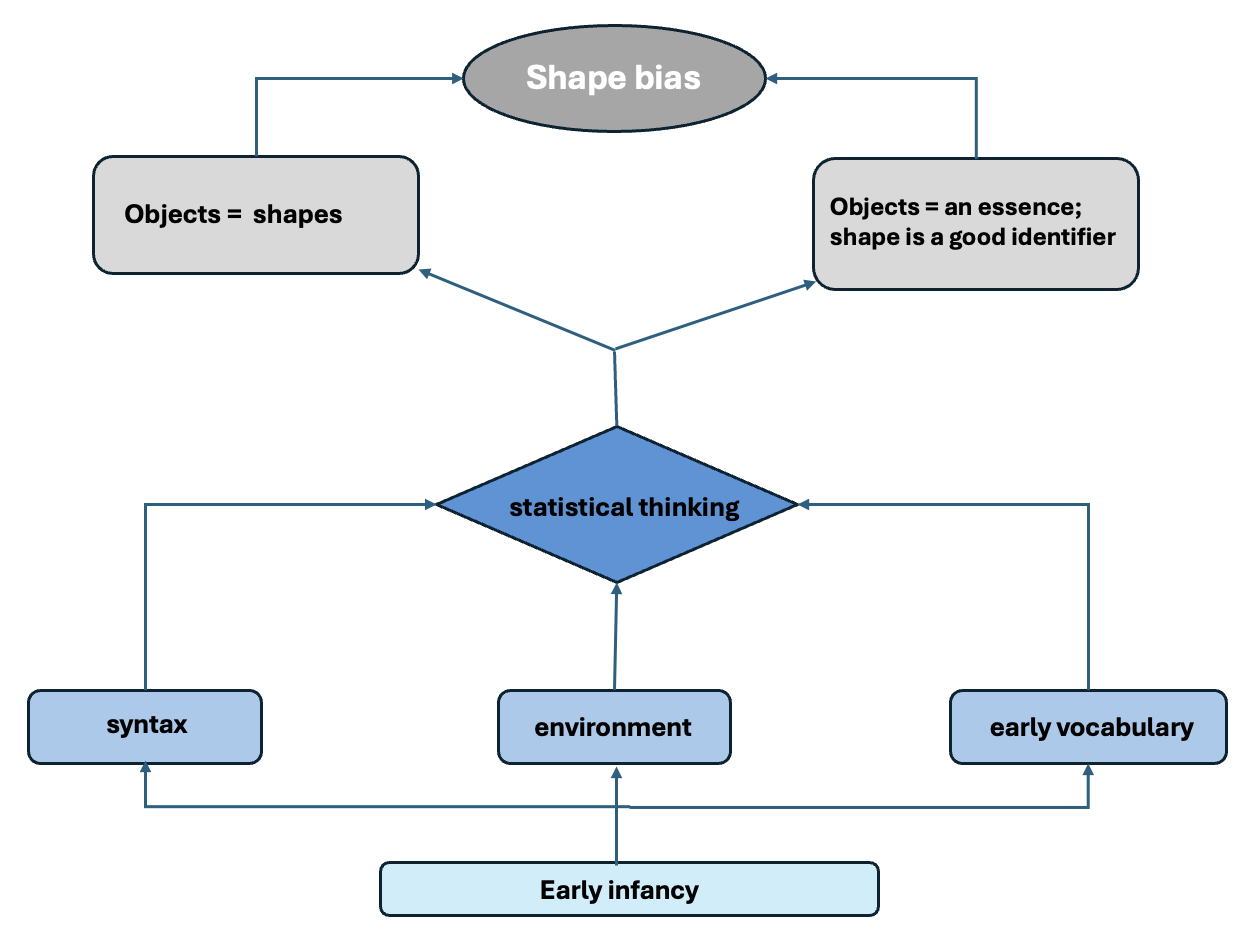
\includegraphics[width=1\linewidth]{conceptual_diagram1} \caption[A diagram to visualize different factors that potentially contribute to the emergence of the shape bias]{A diagram to visualize different factors that potentially contribute to the emergence of the shape bias}\label{fig:flow_diagram }
\end{figure}
\end{CodeChunk}

\subsection{The nature of Knowledge}\label{the-nature-of-knowledge}

Given that task design is influenced by theoretical assumptions, this
raises another important question: What type of knowledge do these tasks
measure? Two key assumptions can stem out of this: Knowledge as Stable
and Fixed: If knowledge is stable, tasks merely elicit pre-existing
constructs. Investigating heterogeneity would then focus on ensuring
task validity and reliability in capturing the theoretical construct.
Knowledge as Dynamic and Task-Dependent: If knowledge is dynamic,
categorization depends on the interaction between task specifics and
children's behavior. This view suggests that children dynamically select
information sources to organize categories, influenced by the context of
the task and the nature of the stimuli (Cimpian \& Markman, 2005; L.
Samuelson, 2006; Smith, Colunga, \& Yoshida, 2010b, 2010a). If the
second assumption holds, achieving consistency in measures across
studies is crucial to isolating the relevant contextual cues that tasks
provide specially for cross-cultural studies that aim to adjudicate
theoretical debates.

Regardless of which assumption holds, it is necessary to evaluate the
heterogeneity in the word categorization studies which highlights the
importance of methodological consistency and the need to consider the
theoretical premises underlying procedural decisions. Understanding how
these premises shape task designs and influence results is key to
advancing our knowledge of label categorization and concept formation.

\section{Sources of Heterogeneity}\label{sources-of-heterogeneity}

The unexplained variability across studies and experiments are suggested
to be due to procedural variation i.e.~task format and stimuli.

\subsection{Task format}\label{task-format}

Generalization in word learning is assessed by teaching children a novel
label for a novel object, and then test them on the ability to extend it
to other objects that share features like shape, or material, etc, with
the exemplar object. Word extensions are measured via Forced-choice
tasks, which require restrictive generalizations, yes/no endorsement
tasks, allowing broader acceptance of category membership which allows
for different levels of similarity and difference (Landau et al., 1988),
or Open-choice tasks, enabling children to reject all options, which is
interpreted as an indication of an understanding of category membership
that goes beyond shared perceptual features. It is not yet clear how
different tasks affect performance. For example, allowing children to
select ``none of those'' reduces shape bias, especially with complex
objects (Cimpian \& Markman, 2005). The choice of the task format is
often guided by the theoretical framework of the researchers, leading to
what seems like a circular stream of events in which theory informs task
selection, and task selection confirms theory.

\subsection{Stimuli}\label{stimuli}

A significant sources of variation in the word extension findings comes
from differences in stimuli. Just like task format, these methodological
decisions are often driven by theoretical frameworks as well. For
instance, studies focusing on low-level attentional biases typically
emphasize contrasts between shape and other perceptual features, such as
color or material, using stimuli designed to highlight these attributes.
On the other hand, studies investigating conceptual understanding often
include cues related to animacy, such as eyes, shoes, or other salient
features, and use test objects that share multiple dimensions with the
exemplar instead of only one to explore broader conceptual frameworks
(Susan S. Jones \& Smith, 1998; Yoshida \& Smith, 2003b). When
functionality is emphasized, stimuli are often paired with
demonstrations of an affordance, stories, or narratives to contrast
shape with function. Children aged 2 to 5 years are found to prioritize
shape, even when provided with functional information (Centner, 2003;
Graham, Williams, \& Huber, 1999; Landau \& Jones, 1998; Merriman,
Scott, \& Marazita, 1993). However, conflicting evidence shows children
sometimes prioritize function or other cues (Kemler Nelson, 1995; Gelman
\& Medin, 1993; etc.). This variation is linked to factors like whether
test objects were handled or how stimuli were designed (e.g., functional
bases vs.~appended parts). In addition, some studies use pictures or
drawings, while others use physical objects (cite).

Lastly, most studies employ between-subjects designs, which do not
control for individual differences, further amplifying heterogeneity.
These procedural and stimuli variations reflect broader theoretical
questions about the origins of the shape bias (Smith \& Medin, 1981). Is
it a Low-level attentional mechanisms driven by attentional processes
that guide children to perceptual features associated with category
labels? Or a Top-down conceptual processes in which the perceptual
features act as identifiers rather than defining properties? Where
should the line be drawn between perceptual feature identification and
the core representation of conceptual labels? Are these separate
processes, or do they exist on a continuum that develops as children
acquire more information? How do attention to perceptual attributes and
conceptual understanding interact during development (Madole \& Oakes,
1999)? These foundational questions influence procedural decisions and
should be kept in mind when investigating label categorization and
concept formation.

\section{Current Study}\label{current-study}

This project seeks to evaluate procedural sources of variability as part
of a larger scale assessment of word generalization across age groups
and languages. We utilize a within-subject design, controlling for
individual differences which we believe is important for a proper
comparison between conditions that require giving different instructions
and cues to the participants. We aim to recruit a larger sample size of
a wider age group, with a variety of items and test trials. Given our
focus on early language acquisition and the noun bias dominating early
vocabulary (Frank, Braginsky, Yurovsky, \& Marchman, 2021), we
prioritize studies examining functional information over other types of
conceptual knowledge.

\subsection{Stimuli design}\label{stimuli-design}

To investigate children's reasoning about objects' properties and
functions, a series of object sets were designed, each containing one
exemplar, a material match, a shape match, a function match, and a
distractor (e.g., dax, fep, blicket, gorp, zimbo, wap, blint). These
sets allowed for systematic manipulation of object features to assess
various cognitive processes related to word learning and category
generalization. In Experiment 1, the shape match was contrasted with a
material match. This served as a baseline check and replication of prior
findings regarding shape bias in categorization tasks. In Experiment 2,
the same exemplar was used, but the shape match was contrasted with a
function match.

\begin{CodeChunk}
\begin{figure}[tb]
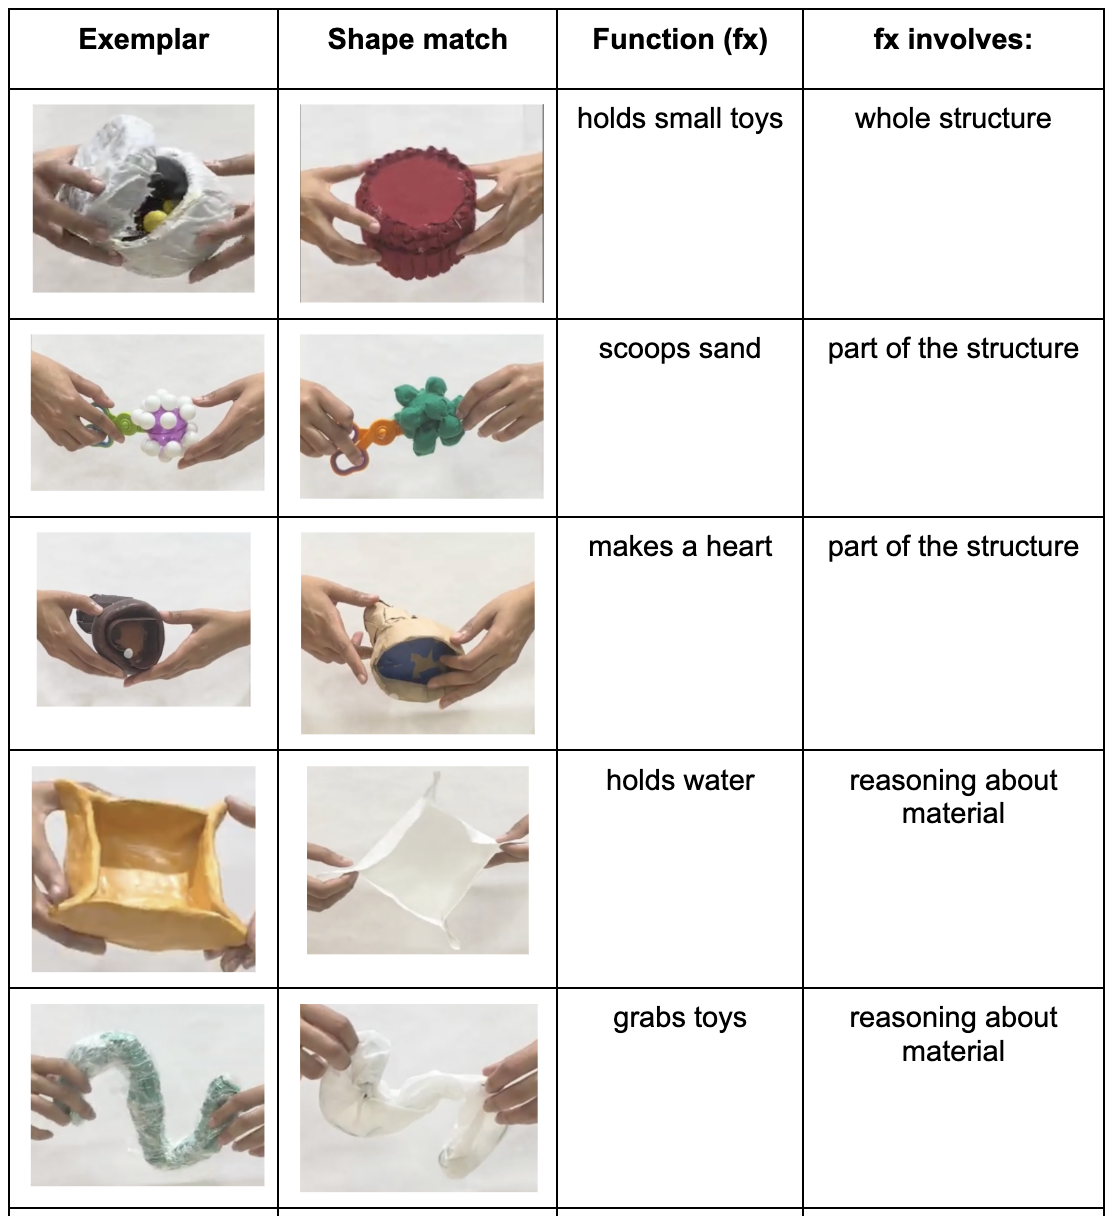
\includegraphics[width=1\linewidth]{stimuli} \caption[A diagram to visualize different factors that potentially contribute to the emergence of the shape bias]{A diagram to visualize different factors that potentially contribute to the emergence of the shape bias}\label{fig:stimulipics }
\end{figure}
\end{CodeChunk}

The function test object was modified in a way that preserved its shape
but altered its functionality (e.g., an object wrapped entirely vs.~one
that could clearly open). Color was excluded across all objects to
ensure that visual similarity was driven solely by shape, material, and
functional cues. Objects were crafted to explore how children reason
about similarity based on whole-object vs.~part-based features (e.g.,
whether specific parts afford a function). Some objects, like the
``Fep,'' ``blint,'' and ``wap,'' were designed with material-critical
functions (e.g., holding water while made of a paper towel). This design
tested whether children could prioritize material when reasoning about
function and to capture the developmental changes. The degree to which
object affordances were visually apparent varied across designs. For
example, The ``Zimbo'' was designed to afford functionality only through
a specific part, while the overall structure was irrelevant. The
``Gorp'' was modeled to resemble objects familiar to slightly older
children, like scissors, allowing exploration of prior experiences'
influence on categorization. This variability was accounted for using
mixed-effects modeling, enabling the examination of how children's
responses were influenced by object features and individual differences.
(An adult similarity rating experiment is currently underway to measure
perceived similarity between objects.)

\section{Experiment 1:}\label{experiment-1}

\subsection{Participants}\label{participants}

Twenty four typically developing English speaking participants (2-5
years old, mean=44.05, SD=15.29) were recruited from a local nursery
school and children's museum in the US (preregistration link).

\subsection{Procedure}\label{procedure}

Seven trials were conducted in which each participant sees an object
being labeled ``this is a dax'', the object is taken away but still in
view, both test objects and the distractor are displayed simultaneously
while asking the child ``can you find another dax by pointing to it?''.
The child gets to hear the label 3 times while viewing it without
touching it.

\begin{CodeChunk}
\begin{figure}[tb]
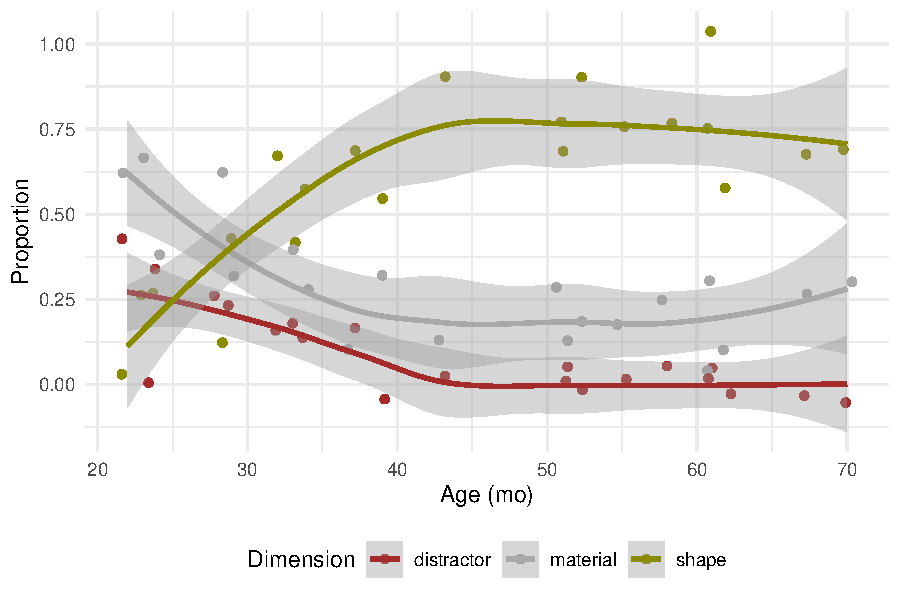
\includegraphics[width=1\linewidth]{figs/first_exp-1} \caption[Developmental trend of choosing by each dimension]{Developmental trend of choosing by each dimension. Smoothed lines are standard error}\label{fig:first_exp}
\end{figure}
\end{CodeChunk}

\begin{CodeChunk}
\begin{figure}[tb]
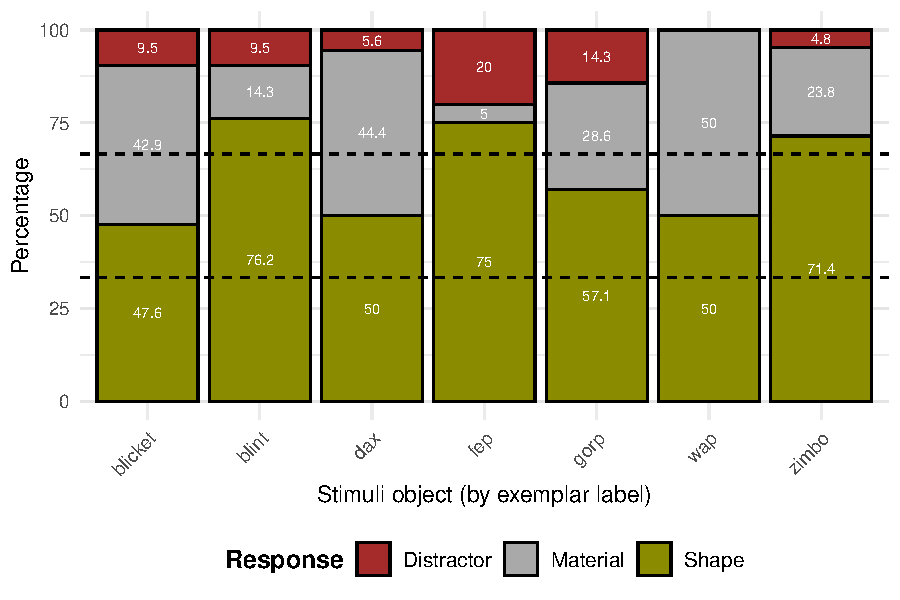
\includegraphics[width=1\linewidth]{figs/first_exp_stim-1} \caption[Percentage of choosing by dimension per stimuli item]{Percentage of choosing by dimension per stimuli item. Dashed line is chance level = 33.3\% }\label{fig:first_exp_stim}
\end{figure}
\end{CodeChunk}

\subsection{Analysis}\label{analysis}

We use a generalized logistic mixed effects model predicting a binary
outcome of choosing by shape. Random intercepts at the level of both
participants and stimuli objects.

\subsection{Results}\label{results}

Participants showed an overall shape bias across all trials (shape:61\%,
material:30\%, distractor: 9\%). Figure \ref{fig:first_exp} shows a
developmental shift to choose by shape by age 3, replicating what is
seen previously in the literature.\\
A generalized logistic mixed-effects model (GLMM) reveals an average
intercept odds of 0.11 (odds of 0.11:1 at the mean age, \(p=\)
\textless{} .001), with a significant increase in odds of 1.06 per unit
increase in age (\(p=\) \textless{} .001). The model also shows
variability at the item-level intercept (variance = 0.11, SD = 0.32)
across 7 unique items (standardlabel groups).

\subsection{Discussion:}\label{discussion}

Overall, even within this small sample of children between 2 and 5 years
of age, data from this experiment confirmed the robustness of the shape
bias. Although the reason why the younger group of kids i.e.~below 3,
chose more by material is not clear now, however, we see variability at
the item level such that for three objects ``blicket, dax, and wap'' we
see an above chance material choices when collapsing across ages. After
replicating the shape bias effect using the set of stimuli we created in
a simple set up, our next experiment explores a design that tests for
two conditions. The first is when shape is only contrasted with material
without any additional information. The second is a condition in which
shape is contrasted with function after demonstrating the function for
the exemplar, while controlling for individual differences with a bigger
sample size to capture variability at the item level as well as any
potential individual differences.

\section{Experiment 2}\label{experiment-2}

\subsection{Participants}\label{participants-1}

31 (target n=96, 24 per each age group) participants between 2-5 years
old (mean=48.22, SD=5.54, n per age group) were recruited from a local
nursery school in the US.

\subsection{Procedure}\label{procedure-1}

A within subject manipulation with two conditions: material or function.
The material condition is identical to the first experiment. In the
function condition, the experimenter introduce the exemplar object
``this is a dax'', gives the child 15 seconds seconds to play with it,
provides functional information `` the dax grapes toys'', gives another
15 seconds to play with it, and puts the toy away but within view,
before introducing the test objects and asks for a response.

\begin{CodeChunk}
\begin{figure*}[!h]
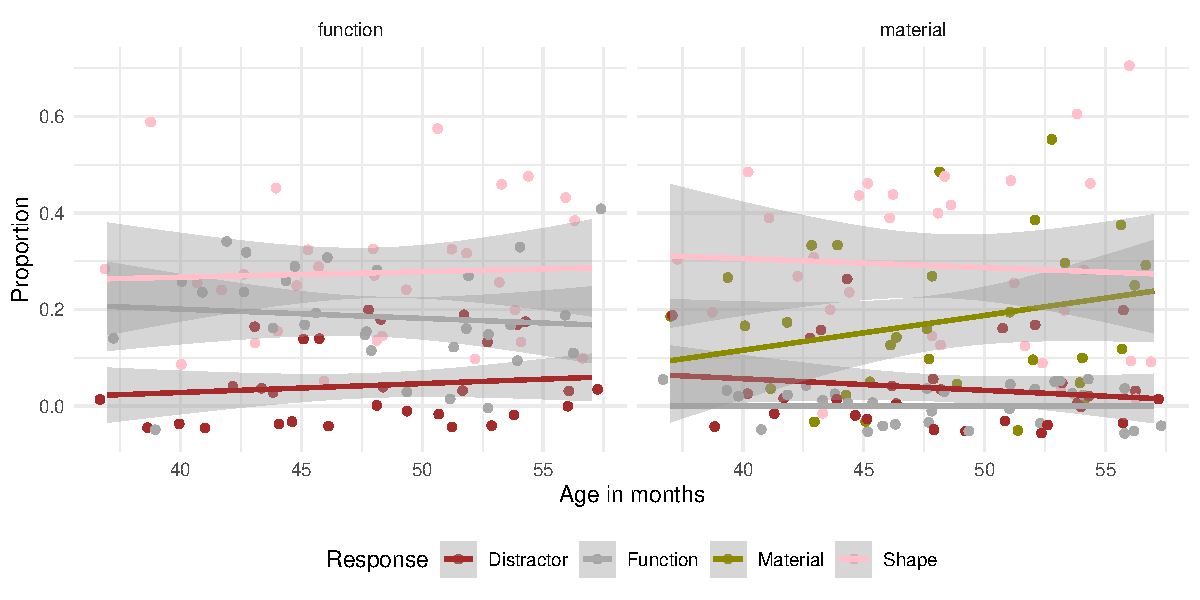
\includegraphics[width=1\linewidth]{figs/jitter_function-1} \caption[Experiment 2, function vs]{Experiment 2, function vs. no function 'material'  condition. Children choose by shape more, even when function information is made salient}\label{fig:jitter_function}
\end{figure*}
\end{CodeChunk}

\begin{CodeChunk}
\begin{figure}[tb]
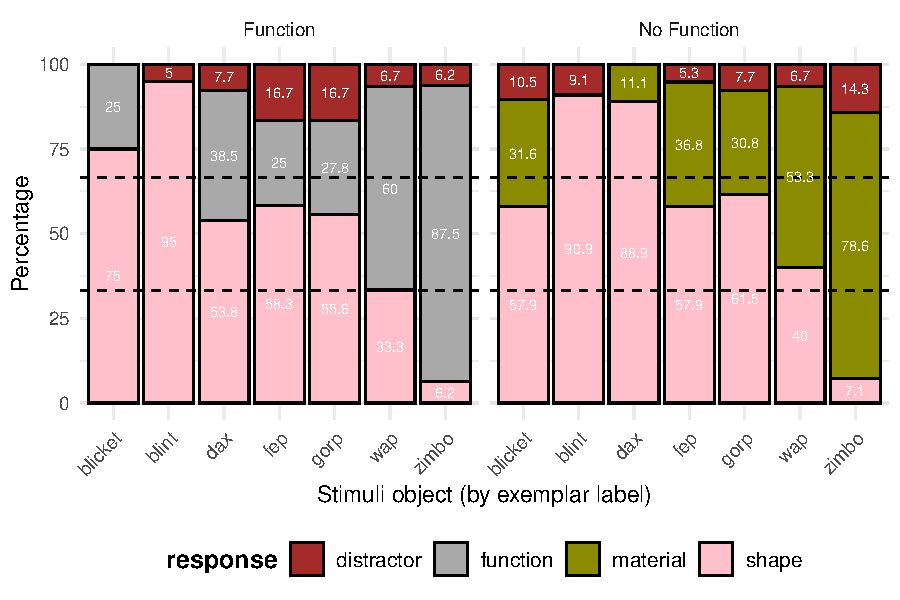
\includegraphics[width=1\linewidth]{figs/sec_exp_stim-1} \caption[Experiment 2, proportion of choosing by each dimension per exemplar item 'indicated by its novel label]{Experiment 2, proportion of choosing by each dimension per exemplar item 'indicated by its novel label. We note variability across items}\label{fig:sec_exp_stim}
\end{figure}
\end{CodeChunk}

\subsection{Preliminary results}\label{preliminary-results}

Similar to what is conveyed in Figure \ref{fig:jitter_function}, a
generalized logistic mixed-effects model (GLMM) showed a lower baseline
odds of the shape bias in the material condition compared to the
function, and the odds ratio increases with age. In additon, random
effects indicate variability in intercepts across participants (SD =
0.22) and across items (SD = 1.38) for 31 participants and 7 items as in
Figure \ref{fig:sec_exp_stim}. (Notably, the confidence intervals show
uncertainty ``include 0'', however data collection is still ongoing.)

\section{Discussion}\label{discussion-1}

The word extension and category organization literature is highly
heterogeneous. Studies in this domain lack an integrative and
commensurable design, which hinders our ability to draw consistent
conclusions. To achieve a more accurate measurement of category
organization and concept learning, we need a reliable and valid range
set of stimuli objects, consistent task formats and test designs, as
well as multi-site cross-cultural experiments unified across
laboratories to maximally account for the variability. Our evaluation of
the word extension literature reveals that making procedural decisions,
which we think are likely a primary source of unexplained variability,
is unattianable without running a series of controlled experiments that
would allow us to systematically assess how different designs and
stimuli covary with response patterns.

In our preliminary results, we see a tendency to generalize by shape,
even in conditions designed to make function salient. This suggests
that, even with a potential saliency effect, where the trials
highlighted functional information, it failed to override the preference
for shape-based choices. In addition, many children explored whether
their chosen test object could perform the intended function after
selecting it based on shape. This behavior implies that the shape-based
selection might not reflect a disregard for functional information but
rather a hypothesis that objects sharing shape might also share
functionality (for example, in the case of the dax, which is a box with
lid that you can use to store small toys, kids choose another box that
is wrapped all over to indicate impossibilty to open, and they still try
to open it afterwards). Meanwhile, in the case of the (gorp), for which
the function wasn't as ambiguous (scooping sand requires the structure
of the object to have two parts that can split and then close to hold
sand inside), in this case the test object was designed in a way that
makes it very clear to not open, hence they went for the function test
choice (see suplementary material). For evaulating the children's
ability to reason about intrinsic affordances, we created the ``Fep'' in
a way such that the material itself is very critical for performing the
function ``holding water while being made of paper towel''. We believe
all these structural differences between objects can explain part of the
variation when we have enough data to fit the model.

As we mentioned in the introduction, procedural variation observed in
the literature have followed theoretical debates and in fact reinforced
by them. We think this endeavor is one step towards achieving validity
and reliability in word extension tasks, as well as discussing
theoretical implications that follow for them. To illusatrate, the
definition of the shape bias construct as a word extension strategy has
been ambiguous and it is also influenced by theoretical framing. For
example, if it is a product of different contingencies and statistical
regularities, it would make sense from a signal detection point of view,
to predict that it will have a graded degree between population,
individuals, and items. Hence, analyzing data on an aggregate level
across all these dimensions hasn't helped advancing our understanding of
cross cultural differences at a theoretical level. We believe, providing
a quantifiable assessment of data across items, individuals, and
building upon that across cultures, will be the only way to resolve
these issues.

\section{References}\label{references}

\setlength{\parindent}{-0.1in} 
\setlength{\leftskip}{0.125in}

\noindent

\phantomsection\label{refs}
\begin{CSLReferences}{1}{0}
\bibitem[\citeproctext]{ref-abdelrahim_frank_2024}
Abdelrahim, S., \& Frank, M. C. (2024, September). Examining the
robustness and generalizability of the shape bias: A meta-analysis.
PsyArXiv.
http://doi.org/\href{https://doi.org/10.31234/osf.io/3by54}{10.31234/osf.io/3by54}

\bibitem[\citeproctext]{ref-Baldwin1992ClarifyingTR}
Baldwin, D. A. (1992). Clarifying the role of shape in children's
taxonomic assumption. \emph{Journal of Experimental Child Psychology},
\emph{54 3}, 392--416. Retrieved from
\url{https://api.semanticscholar.org/CorpusID:29725812}

\bibitem[\citeproctext]{ref-BOOTH2002B11}
Booth, A. E., \& Waxman, S. R. (2002). Word learning is {``smart''}:
Evidence that conceptual information affects preschoolers' extension of
novel words. \emph{Cognition}, \emph{84}(1), B11--B22.
http://doi.org/\url{https://doi.org/10.1016/S0010-0277(02)00015-X}

\bibitem[\citeproctext]{ref-dejavu}
Booth, A., \& Waxman, S. (2006). Déjà vu all over again: Re-revisiting
the conceptual status of early word learning: Comment on smith and
samuelson (2006). \emph{Developmental Psychology}, \emph{42}, 1344--6.
http://doi.org/\href{https://doi.org/10.1037/0012-1649.42.6.1344}{10.1037/0012-1649.42.6.1344}

\bibitem[\citeproctext]{ref-2005_Booth}
Booth, A., Waxman, S., \& Huang, Y. (2005). Conceptual information
permeates word learning in infancy. \emph{Developmental Psychology},
\emph{41}(3), 491--505.
http://doi.org/\href{https://doi.org/10.1037/0012-1649.41.3.491}{10.1037/0012-1649.41.3.491}

\bibitem[\citeproctext]{ref-Bruner1964TheCO}
Bruner, J. S. (1964). The course of cognitive growth. \emph{American
Psychologist}, \emph{19}, 1--15. Retrieved from
\url{https://api.semanticscholar.org/CorpusID:145196722}

\bibitem[\citeproctext]{ref-Centner2003OnRM}
Centner, D. (2003). On relational meaning : The acquisition of verb
meaning. In. Retrieved from
\url{https://api.semanticscholar.org/CorpusID:7539638}

\bibitem[\citeproctext]{ref-cimpian2005absence}
Cimpian, A., \& Markman, E. M. (2005). The absence of a shape bias in
children's word learning. \emph{Developmental Psychology}, \emph{41}(6),
1003.

\bibitem[\citeproctext]{ref-CLARK197365}
CLARK, E. V. (1973). WHAT's IN a WORD? ON THE CHILD's ACQUISITION OF
SEMANTICS IN HIS FIRST LANGUAGE11This research was supported in part by
NSF grant GS-1880 to the language universals project, stanford
university, and in part by NSF grant GS-30040 to the author. In T. E.
Moore (Ed.), \emph{Cognitive development and acquisition of language}
(pp. 65--110). San Diego: Academic Press.
http://doi.org/\url{https://doi.org/10.1016/B978-0-12-505850-6.50009-8}

\bibitem[\citeproctext]{ref-colunga2000learning}
Colunga, E., \& Smith, L. B. (2000). Learning to learn words: A
cross-linguistic study of the shape and material biases. In
\emph{Proceedings of the 24th annual boston university conference on
language development} (Vol. 1, pp. 197--207).

\bibitem[\citeproctext]{ref-frank2021}
Frank, M. C., Braginsky, M., Yurovsky, D., \& Marchman, V. A. (2021).
\emph{Variability and consistency in early language learning: The
wordbank project}. The MIT Press.
http://doi.org/\href{https://doi.org/10.7551/mitpress/11577.001.0001}{10.7551/mitpress/11577.001.0001}

\bibitem[\citeproctext]{ref-gathercole_1997}
Gathercole, V. C. M., \& Min, H. (1997). Word meaning biases or
language-specific effects? {Evidence} from {English}, {Spanish} and
{Korean}. \emph{First Language}, \emph{17}(51), 031--56.
http://doi.org/\href{https://doi.org/10.1177/014272379701705102}{10.1177/014272379701705102}

\bibitem[\citeproctext]{ref-gershkoff2004shape}
Gershkoff-Stowe, L., \& Smith, L. B. (2004). Shape and the first hundred
nouns. \emph{Child Development}, \emph{75}(4), 1098--1114.

\bibitem[\citeproctext]{ref-graham_2010}
Graham, S. A., \& Diesendruck, G. (2010). Fifteen-month-old infants
attend to shape over other perceptual properties in an induction task.
\emph{Cognitive Development}, \emph{25}(2), 111--123.
http://doi.org/\href{https://doi.org/10.1016/j.cogdev.2009.06.002}{10.1016/j.cogdev.2009.06.002}

\bibitem[\citeproctext]{ref-Graham1999InfantsRO}
Graham, S. A., \& Poulin-Dubois, D. (1999). Infants' reliance on shape
to generalize novel labels to animate and inanimate objects.
\emph{Journal of Child Language}, \emph{26}, 295--320. Retrieved from
\url{https://api.semanticscholar.org/CorpusID:43424185}

\bibitem[\citeproctext]{ref-GRAHAM1999128}
Graham, S. A., Williams, L. D., \& Huber, J. F. (1999). Preschoolers'
and adults' reliance on object shape and object function for lexical
extension. \emph{Journal of Experimental Child Psychology},
\emph{74}(2), 128--151.
http://doi.org/\url{https://doi.org/10.1006/jecp.1999.2514}

\bibitem[\citeproctext]{ref-imai1997}
Imai, M., \& Gentner, D. (1997). A cross-linguistic study of early word
meaning: Universal ontology and linguistic influence. \emph{Cognition},
\emph{62}(2), 169--200.

\bibitem[\citeproctext]{ref-imai_childrens_1994}
Imai, M., Gentner, D., \& Uchida, N. (1994). Children's theories of word
meaning: {The} role of shape similarity in early acquisition.
\emph{Cognitive Development}, \emph{9}(1), 45--75.
http://doi.org/\href{https://doi.org/10.1016/0885-2014(94)90019-1}{10.1016/0885-2014(94)90019-1}

\bibitem[\citeproctext]{ref-jara2022}
Jara-Ettinger, J., Levy, R., Sakel, J., Huanca, T., \& Gibson, E.
(2022). The origins of the shape bias: Evidence from the tsimane'.
\emph{Journal of Experimental Psychology: General}.

\bibitem[\citeproctext]{ref-Jones2003}
Jones, Susan S. (2003). Late talkers show no shape bias in a novel name
extension task. \emph{Developmental Science}, \emph{6}(5), 477--483.
http://doi.org/\url{https://doi.org/10.1111/1467-7687.00304}

\bibitem[\citeproctext]{ref-JONES1993113}
Jones, Susan S., \& Smith, L. B. (1993). The place of perception in
children's concepts. \emph{Cognitive Development}, \emph{8}(2),
113--139.
http://doi.org/\url{https://doi.org/10.1016/0885-2014(93)90008-S}

\bibitem[\citeproctext]{ref-JONES1998323}
Jones, Susan S., \& Smith, L. B. (1998). How children name objects with
shoes. \emph{Cognitive Development}, \emph{13}(3), 323--334.
http://doi.org/\url{https://doi.org/10.1016/S0885-2014(98)90014-4}

\bibitem[\citeproctext]{ref-JONES_SMITH_2005}
JONES, S. S., \& SMITH, L. B. (2005). Object name learning and object
perception: A deficit in late talkers. \emph{Journal of Child Language},
\emph{32}(1), 223--240.
http://doi.org/\href{https://doi.org/10.1017/S0305000904006646}{10.1017/S0305000904006646}

\bibitem[\citeproctext]{ref-Kucker2019ReproducibilityAA}
Kucker, S. C., Samuelson, L. K., Perry, L. K., Yoshida, H., Colunga, E.,
Lorenz, M. G., \& Smith, L. B. (2019). Reproducibility and a unifying
explanation: Lessons from the shape bias. \emph{Infant Behavior \&
Development}, \emph{54}, 156--165. Retrieved from
\url{https://api.semanticscholar.org/CorpusID:53045726}

\bibitem[\citeproctext]{ref-landau1996}
Landau, B., \& Jones, S. (1998). Object shape, object function, and
object name. \emph{Journal of Memory and Language - J MEM LANG},
\emph{38}, 1--27.
http://doi.org/\href{https://doi.org/10.1006/jmla.1997.2533}{10.1006/jmla.1997.2533}

\bibitem[\citeproctext]{ref-LANDAU1988299}
Landau, B., Smith, L. B., \& Jones, S. S. (1988). The importance of
shape in early lexical learning. \emph{Cognitive Development},
\emph{3}(3), 299--321.
http://doi.org/\url{https://doi.org/10.1016/0885-2014(88)90014-7}

\bibitem[\citeproctext]{ref-Merriman_Scott_Marazita_1993}
Merriman, W. E., Scott, P. D., \& Marazita, J. (1993). An
appearance-function shift in children's object naming. \emph{Journal of
Child Language}, \emph{20}(1), 101--118.
http://doi.org/\href{https://doi.org/10.1017/S0305000900009144}{10.1017/S0305000900009144}

\bibitem[\citeproctext]{ref-Nelson1974ConceptWA}
Nelson, K. (1974). Concept, word, and sentence: Interrelations in
acquisition and development. \emph{Psychological Review}, \emph{81},
267--285. Retrieved from
\url{https://api.semanticscholar.org/CorpusID:143965074}

\bibitem[\citeproctext]{ref-perry2010learn}
Perry, L. K., Samuelson, L. K., Malloy, L. M., \& Schiffer, R. N.
(2010). Learn locally, think globally: Exemplar variability supports
higher-order generalization and word learning. \emph{Psychological
Science}, \emph{21}(12), 1894--1902.

\bibitem[\citeproctext]{ref-replycimpian}
Samuelson, L. (2006). An attentional learning account of the shape bias:
Reply to cimpian and markman (2005) and booth, waxman, and huang (2005).
\emph{Developmental Psychology}, \emph{42}, 1339--43.
http://doi.org/\href{https://doi.org/10.1037/0012-1649.42.6.1339}{10.1037/0012-1649.42.6.1339}

\bibitem[\citeproctext]{ref-samuelson_statistical_2002}
Samuelson, Larissa K. (2002). Statistical regularities in vocabulary
guide language acquisition in connectionist models and 15-20-month-olds.
\emph{Developmental Psychology}, \emph{38}(6), 1016--1037.
http://doi.org/\href{https://doi.org/10.1037/0012-1649.38.6.1016}{10.1037/0012-1649.38.6.1016}

\bibitem[\citeproctext]{ref-2005_Samuelson}
Samuelson, Larissa K. (2005). Statistical regularities in vocabulary
guide language acquisition in connectionist models and 15-20-month-olds.
\emph{Developmental Psychology}, \emph{38}(6), 1016--1037.
http://doi.org/\href{https://doi.org/10.1037/0012-1649.38.6.1016}{10.1037/0012-1649.38.6.1016}

\bibitem[\citeproctext]{ref-samuelson2008rigid}
Samuelson, Larissa K., Horst, J. S., Schutte, A. R., \& Dobbertin, B. N.
(2008). Rigid thinking about deformables: Do children sometimes
overgeneralize the shape bias? \emph{Journal of Child Language},
\emph{35}(3), 559--589.

\bibitem[\citeproctext]{ref-SAMUELSON2010138}
Samuelson, Larissa K., \& Perone, S. (2010). Rethinking
conceptually-based inference --- grounding representation in task and
behavioral dynamics: Commentary on {``fifteen-month-old infants attend
to shape over other perceptual properties in an induction task,''} by s.
Graham and g. Diesendruck, and {``form follows function: Learning about
function helps children learn about shape,''} by e. Ware and a. booth.
\emph{Cognitive Development}, \emph{25}(2), 138--148.
http://doi.org/\url{https://doi.org/10.1016/j.cogdev.2010.02.002}

\bibitem[\citeproctext]{ref-samuelson1999}
Samuelson, Larissa K., \& Smith, L. B. (1999). Early noun vocabularies:
Do ontology, category structure and syntax correspond? \emph{Cognition},
\emph{73}(1), 1--33.

\bibitem[\citeproctext]{ref-samuelson2000children}
Samuelson, Larissa K., \& Smith, L. B. (2000). Children's attention to
rigid and deformable shape in naming and non-naming tasks. \emph{Child
Development}, \emph{71}(6), 1555--1570.

\bibitem[\citeproctext]{ref-dynamicBias}
Samuelson, L., \& Horst, J. (2008). Shape bias special section:
Confronting complexity: Insights from the details of behavior over
multiple timescales. \emph{Developmental Science}, \emph{11}, 209--15.
http://doi.org/\href{https://doi.org/10.1111/j.1467-7687.2007.00667.x}{10.1111/j.1467-7687.2007.00667.x}

\bibitem[\citeproctext]{ref-Smith2003MakingAO}
Smith, L. B., Colunga, E., \& Yoshida, H. (2003). Making an ontology:
Cross-linguistic evidence. In. Retrieved from
\url{https://api.semanticscholar.org/CorpusID:195941919}

\bibitem[\citeproctext]{ref-smithcolunga2010}
Smith, L. B., Colunga, E., \& Yoshida, H. (2010a). Knowledge as process:
Contextually cued attention and early word learning. \emph{Cognitive
Science}, \emph{34}(7), 1287--1314.
http://doi.org/\url{https://doi.org/10.1111/j.1551-6709.2010.01130.x}

\bibitem[\citeproctext]{ref-smithContext}
Smith, L. B., Colunga, E., \& Yoshida, H. (2010b). Knowledge as process:
Contextually cued attention and early word learning. \emph{Cognitive
Science}, \emph{34}(7), 1287--1314.
http://doi.org/\url{https://doi.org/10.1111/j.1551-6709.2010.01130.x}

\bibitem[\citeproctext]{ref-Smith1996NamingIY}
Smith, L. B., Jones, S. S., \& Landau, B. (1996). Naming in young
children: A dumb attentional mechanism? \emph{Cognition}, \emph{60},
143--171. Retrieved from
\url{https://api.semanticscholar.org/CorpusID:18659784}

\bibitem[\citeproctext]{ref-smith_object_2002}
Smith, L. B., Jones, S. S., Landau, B., Gershkoff-Stowe, L., \&
Samuelson, L. (2002). Object name learning provides on-the-job training
for attention. \emph{Psychological Science}, \emph{13}(1), 13--19.
http://doi.org/\href{https://doi.org/10.1111/1467-9280.00403}{10.1111/1467-9280.00403}

\bibitem[\citeproctext]{ref-soja1991ontological}
Soja, Nancy N., Carey, S., \& Spelke, E. S. (1991). Ontological
categories guide young children's inductions of word meaning: Object
terms and substance terms. \emph{Cognition}, \emph{38}(2), 179--211.

\bibitem[\citeproctext]{ref-soja_perception_1992}
Soja, Nancy N., Carey, S., \& Spelke, E. S. (1992). Perception,
ontology, and word meaning. \emph{Cognition}, \emph{45}(1), 101--107.
http://doi.org/\href{https://doi.org/10.1016/0010-0277(92)90025-D}{10.1016/0010-0277(92)90025-D}

\bibitem[\citeproctext]{ref-subrahmanyam_2006}
Subrahmanyam, K., \& Chen, H.-H. N. (2006). A crosslinguistic study of
children's noun learning: {The} case of object and substance words.
\emph{First Language}, \emph{26}(2), 141--160.
http://doi.org/\href{https://doi.org/10.1177/0142723706060744}{10.1177/0142723706060744}

\bibitem[\citeproctext]{ref-TekAutism}
Tek, S., Jaffery, R., Fein, D., \& Naigles, L. (2008). Do children with
autism show a shape bias in word learning? \emph{Autism Research :
Official Journal of the International Society for Autism Research},
\emph{1}, 208--22.
http://doi.org/\href{https://doi.org/10.1002/aur.38}{10.1002/aur.38}

\bibitem[\citeproctext]{ref-TekAutismLessons}
Tek, S., \& Naigles, L. (2017). The shape bias as a word-learning
principle: Lessons from and for autism spectrum disorder.
\emph{Translational Issues in Psychological Science}, \emph{3}, 94--103.
http://doi.org/\href{https://doi.org/10.1037/tps0000104}{10.1037/tps0000104}

\bibitem[\citeproctext]{ref-WARE2010124}
Ware, E. A., \& Booth, A. E. (2010). Form follows function: Learning
about function helps children learn about shape. \emph{Cognitive
Development}, \emph{25}(2), 124--137.
http://doi.org/\url{https://doi.org/10.1016/j.cogdev.2009.10.003}

\bibitem[\citeproctext]{ref-yoshida2003known}
Yoshida, H., \& Smith, L. B. (2003a). Known and novel noun extensions:
Attention at two levels of abstraction. \emph{Child Development},
\emph{74}(2), 564--577.

\bibitem[\citeproctext]{ref-yoshida2003}
Yoshida, H., \& Smith, L. B. (2003b). Shifting ontological boundaries:
How japanese- and english-speaking children generalize names for animals
and artifacts. \emph{Developmental Science}, \emph{6}(1), 1--17.
http://doi.org/\url{https://doi.org/10.1111/1467-7687.00247/_1}

\end{CSLReferences}

\bibliographystyle{apacite}


\end{document}
